% Options for packages loaded elsewhere
\PassOptionsToPackage{unicode}{hyperref}
\PassOptionsToPackage{hyphens}{url}
%
\documentclass[
  ignorenonframetext,
]{beamer}
\usepackage{pgfpages}
\setbeamertemplate{caption}[numbered]
\setbeamertemplate{caption label separator}{: }
\setbeamercolor{caption name}{fg=normal text.fg}
\beamertemplatenavigationsymbolsempty
% Prevent slide breaks in the middle of a paragraph
\widowpenalties 1 10000
\raggedbottom
\setbeamertemplate{part page}{
  \centering
  \begin{beamercolorbox}[sep=16pt,center]{part title}
    \usebeamerfont{part title}\insertpart\par
  \end{beamercolorbox}
}
\setbeamertemplate{section page}{
  \centering
  \begin{beamercolorbox}[sep=12pt,center]{part title}
    \usebeamerfont{section title}\insertsection\par
  \end{beamercolorbox}
}
\setbeamertemplate{subsection page}{
  \centering
  \begin{beamercolorbox}[sep=8pt,center]{part title}
    \usebeamerfont{subsection title}\insertsubsection\par
  \end{beamercolorbox}
}
\AtBeginPart{
  \frame{\partpage}
}
\AtBeginSection{
  \ifbibliography
  \else
    \frame{\sectionpage}
  \fi
}
\AtBeginSubsection{
  \frame{\subsectionpage}
}

\usepackage{amsmath,amssymb}
\usepackage{lmodern}
\usepackage{iftex}
\ifPDFTeX
  \usepackage[T1]{fontenc}
  \usepackage[utf8]{inputenc}
  \usepackage{textcomp} % provide euro and other symbols
\else % if luatex or xetex
  \usepackage{unicode-math}
  \defaultfontfeatures{Scale=MatchLowercase}
  \defaultfontfeatures[\rmfamily]{Ligatures=TeX,Scale=1}
\fi
% Use upquote if available, for straight quotes in verbatim environments
\IfFileExists{upquote.sty}{\usepackage{upquote}}{}
\IfFileExists{microtype.sty}{% use microtype if available
  \usepackage[]{microtype}
  \UseMicrotypeSet[protrusion]{basicmath} % disable protrusion for tt fonts
}{}
\makeatletter
\@ifundefined{KOMAClassName}{% if non-KOMA class
  \IfFileExists{parskip.sty}{%
    \usepackage{parskip}
  }{% else
    \setlength{\parindent}{0pt}
    \setlength{\parskip}{6pt plus 2pt minus 1pt}}
}{% if KOMA class
  \KOMAoptions{parskip=half}}
\makeatother
\usepackage{xcolor}
\newif\ifbibliography
\setlength{\emergencystretch}{3em} % prevent overfull lines
\setcounter{secnumdepth}{-\maxdimen} % remove section numbering

\usepackage{color}
\usepackage{fancyvrb}
\newcommand{\VerbBar}{|}
\newcommand{\VERB}{\Verb[commandchars=\\\{\}]}
\DefineVerbatimEnvironment{Highlighting}{Verbatim}{commandchars=\\\{\}}
% Add ',fontsize=\small' for more characters per line
\usepackage{framed}
\definecolor{shadecolor}{RGB}{241,243,245}
\newenvironment{Shaded}{\begin{snugshade}}{\end{snugshade}}
\newcommand{\AlertTok}[1]{\textcolor[rgb]{0.68,0.00,0.00}{#1}}
\newcommand{\AnnotationTok}[1]{\textcolor[rgb]{0.37,0.37,0.37}{#1}}
\newcommand{\AttributeTok}[1]{\textcolor[rgb]{0.40,0.45,0.13}{#1}}
\newcommand{\BaseNTok}[1]{\textcolor[rgb]{0.68,0.00,0.00}{#1}}
\newcommand{\BuiltInTok}[1]{\textcolor[rgb]{0.00,0.23,0.31}{#1}}
\newcommand{\CharTok}[1]{\textcolor[rgb]{0.13,0.47,0.30}{#1}}
\newcommand{\CommentTok}[1]{\textcolor[rgb]{0.37,0.37,0.37}{#1}}
\newcommand{\CommentVarTok}[1]{\textcolor[rgb]{0.37,0.37,0.37}{\textit{#1}}}
\newcommand{\ConstantTok}[1]{\textcolor[rgb]{0.56,0.35,0.01}{#1}}
\newcommand{\ControlFlowTok}[1]{\textcolor[rgb]{0.00,0.23,0.31}{#1}}
\newcommand{\DataTypeTok}[1]{\textcolor[rgb]{0.68,0.00,0.00}{#1}}
\newcommand{\DecValTok}[1]{\textcolor[rgb]{0.68,0.00,0.00}{#1}}
\newcommand{\DocumentationTok}[1]{\textcolor[rgb]{0.37,0.37,0.37}{\textit{#1}}}
\newcommand{\ErrorTok}[1]{\textcolor[rgb]{0.68,0.00,0.00}{#1}}
\newcommand{\ExtensionTok}[1]{\textcolor[rgb]{0.00,0.23,0.31}{#1}}
\newcommand{\FloatTok}[1]{\textcolor[rgb]{0.68,0.00,0.00}{#1}}
\newcommand{\FunctionTok}[1]{\textcolor[rgb]{0.28,0.35,0.67}{#1}}
\newcommand{\ImportTok}[1]{\textcolor[rgb]{0.00,0.46,0.62}{#1}}
\newcommand{\InformationTok}[1]{\textcolor[rgb]{0.37,0.37,0.37}{#1}}
\newcommand{\KeywordTok}[1]{\textcolor[rgb]{0.00,0.23,0.31}{#1}}
\newcommand{\NormalTok}[1]{\textcolor[rgb]{0.00,0.23,0.31}{#1}}
\newcommand{\OperatorTok}[1]{\textcolor[rgb]{0.37,0.37,0.37}{#1}}
\newcommand{\OtherTok}[1]{\textcolor[rgb]{0.00,0.23,0.31}{#1}}
\newcommand{\PreprocessorTok}[1]{\textcolor[rgb]{0.68,0.00,0.00}{#1}}
\newcommand{\RegionMarkerTok}[1]{\textcolor[rgb]{0.00,0.23,0.31}{#1}}
\newcommand{\SpecialCharTok}[1]{\textcolor[rgb]{0.37,0.37,0.37}{#1}}
\newcommand{\SpecialStringTok}[1]{\textcolor[rgb]{0.13,0.47,0.30}{#1}}
\newcommand{\StringTok}[1]{\textcolor[rgb]{0.13,0.47,0.30}{#1}}
\newcommand{\VariableTok}[1]{\textcolor[rgb]{0.07,0.07,0.07}{#1}}
\newcommand{\VerbatimStringTok}[1]{\textcolor[rgb]{0.13,0.47,0.30}{#1}}
\newcommand{\WarningTok}[1]{\textcolor[rgb]{0.37,0.37,0.37}{\textit{#1}}}

\providecommand{\tightlist}{%
  \setlength{\itemsep}{0pt}\setlength{\parskip}{0pt}}\usepackage{longtable,booktabs,array}
\usepackage{calc} % for calculating minipage widths
\usepackage{caption}
% Make caption package work with longtable
\makeatletter
\def\fnum@table{\tablename~\thetable}
\makeatother
\usepackage{graphicx}
\makeatletter
\def\maxwidth{\ifdim\Gin@nat@width>\linewidth\linewidth\else\Gin@nat@width\fi}
\def\maxheight{\ifdim\Gin@nat@height>\textheight\textheight\else\Gin@nat@height\fi}
\makeatother
% Scale images if necessary, so that they will not overflow the page
% margins by default, and it is still possible to overwrite the defaults
% using explicit options in \includegraphics[width, height, ...]{}
\setkeys{Gin}{width=\maxwidth,height=\maxheight,keepaspectratio}
% Set default figure placement to htbp
\makeatletter
\def\fps@figure{htbp}
\makeatother

\makeatletter
\makeatother
\makeatletter
\makeatother
\makeatletter
\@ifpackageloaded{caption}{}{\usepackage{caption}}
\AtBeginDocument{%
\ifdefined\contentsname
  \renewcommand*\contentsname{Table of contents}
\else
  \newcommand\contentsname{Table of contents}
\fi
\ifdefined\listfigurename
  \renewcommand*\listfigurename{List of Figures}
\else
  \newcommand\listfigurename{List of Figures}
\fi
\ifdefined\listtablename
  \renewcommand*\listtablename{List of Tables}
\else
  \newcommand\listtablename{List of Tables}
\fi
\ifdefined\figurename
  \renewcommand*\figurename{Figure}
\else
  \newcommand\figurename{Figure}
\fi
\ifdefined\tablename
  \renewcommand*\tablename{Table}
\else
  \newcommand\tablename{Table}
\fi
}
\@ifpackageloaded{float}{}{\usepackage{float}}
\floatstyle{ruled}
\@ifundefined{c@chapter}{\newfloat{codelisting}{h}{lop}}{\newfloat{codelisting}{h}{lop}[chapter]}
\floatname{codelisting}{Listing}
\newcommand*\listoflistings{\listof{codelisting}{List of Listings}}
\makeatother
\makeatletter
\@ifpackageloaded{caption}{}{\usepackage{caption}}
\@ifpackageloaded{subcaption}{}{\usepackage{subcaption}}
\makeatother
\makeatletter
\@ifpackageloaded{tcolorbox}{}{\usepackage[many]{tcolorbox}}
\makeatother
\makeatletter
\@ifundefined{shadecolor}{\definecolor{shadecolor}{rgb}{.97, .97, .97}}
\makeatother
\makeatletter
\makeatother
\ifLuaTeX
  \usepackage{selnolig}  % disable illegal ligatures
\fi
\IfFileExists{bookmark.sty}{\usepackage{bookmark}}{\usepackage{hyperref}}
\IfFileExists{xurl.sty}{\usepackage{xurl}}{} % add URL line breaks if available
\urlstyle{same} % disable monospaced font for URLs
\hypersetup{
  hidelinks,
  pdfcreator={LaTeX via pandoc}}

\author{}
\date{}

\begin{document}
\ifdefined\Shaded\renewenvironment{Shaded}{\begin{tcolorbox}[breakable, borderline west={3pt}{0pt}{shadecolor}, sharp corners, interior hidden, enhanced, boxrule=0pt, frame hidden]}{\end{tcolorbox}}\fi

\begin{frame}{Functions}
\protect\hypertarget{functions}{}
\begin{itemize}
\tightlist
\item
  A function is a block of organized, reusable code that is used to
  perform a single, related action. Functions provide better modularity
  for your application and a high degree of code reusing
\end{itemize}
\end{frame}

\begin{frame}[fragile]
\begin{block}{Functions Already used}
\protect\hypertarget{functions-already-used}{}
\begin{Shaded}
\begin{Highlighting}[]
\NormalTok{x }\OtherTok{\textless{}{-}} \DecValTok{1}\SpecialCharTok{:}\DecValTok{10}
\NormalTok{y }\OtherTok{\textless{}{-}} \DecValTok{11}\SpecialCharTok{:}\DecValTok{20}
\FunctionTok{sum}\NormalTok{(x)}
\end{Highlighting}
\end{Shaded}

\begin{verbatim}
[1] 55
\end{verbatim}

\begin{Shaded}
\begin{Highlighting}[]
\FunctionTok{mean}\NormalTok{(x)}
\end{Highlighting}
\end{Shaded}

\begin{verbatim}
[1] 5.5
\end{verbatim}

\begin{Shaded}
\begin{Highlighting}[]
\FunctionTok{cor}\NormalTok{(x, y)}
\end{Highlighting}
\end{Shaded}

\begin{verbatim}
[1] 1
\end{verbatim}
\end{block}
\end{frame}

\begin{frame}[fragile]
\begin{Shaded}
\begin{Highlighting}[]
\NormalTok{lm\_fit }\OtherTok{\textless{}{-}} \FunctionTok{lm}\NormalTok{(Petal.Length }\SpecialCharTok{\textasciitilde{}}\NormalTok{ Petal.Width, }\AttributeTok{data =}\NormalTok{ iris)}

\FunctionTok{library}\NormalTok{(broom)}
\end{Highlighting}
\end{Shaded}
\end{frame}

\begin{frame}[fragile]
\begin{Shaded}
\begin{Highlighting}[]
\NormalTok{cols }\OtherTok{\textless{}{-}} \FunctionTok{c}\NormalTok{( }\StringTok{"estimate"}\NormalTok{, }\StringTok{"std.error"}\NormalTok{, }\StringTok{"statistic"}\NormalTok{, }\StringTok{"p.value"}\NormalTok{)}
\NormalTok{tidy\_lm }\OtherTok{\textless{}{-}} \FunctionTok{tidy}\NormalTok{(lm\_fit) }
\NormalTok{tidy\_lm }\SpecialCharTok{\%\textgreater{}\%} \FunctionTok{datatable}\NormalTok{() }\SpecialCharTok{\%\textgreater{}\%}
\FunctionTok{formatRound}\NormalTok{(}\AttributeTok{columns =}\NormalTok{ cols,  }\AttributeTok{digits=}\DecValTok{3}\NormalTok{)}
\end{Highlighting}
\end{Shaded}

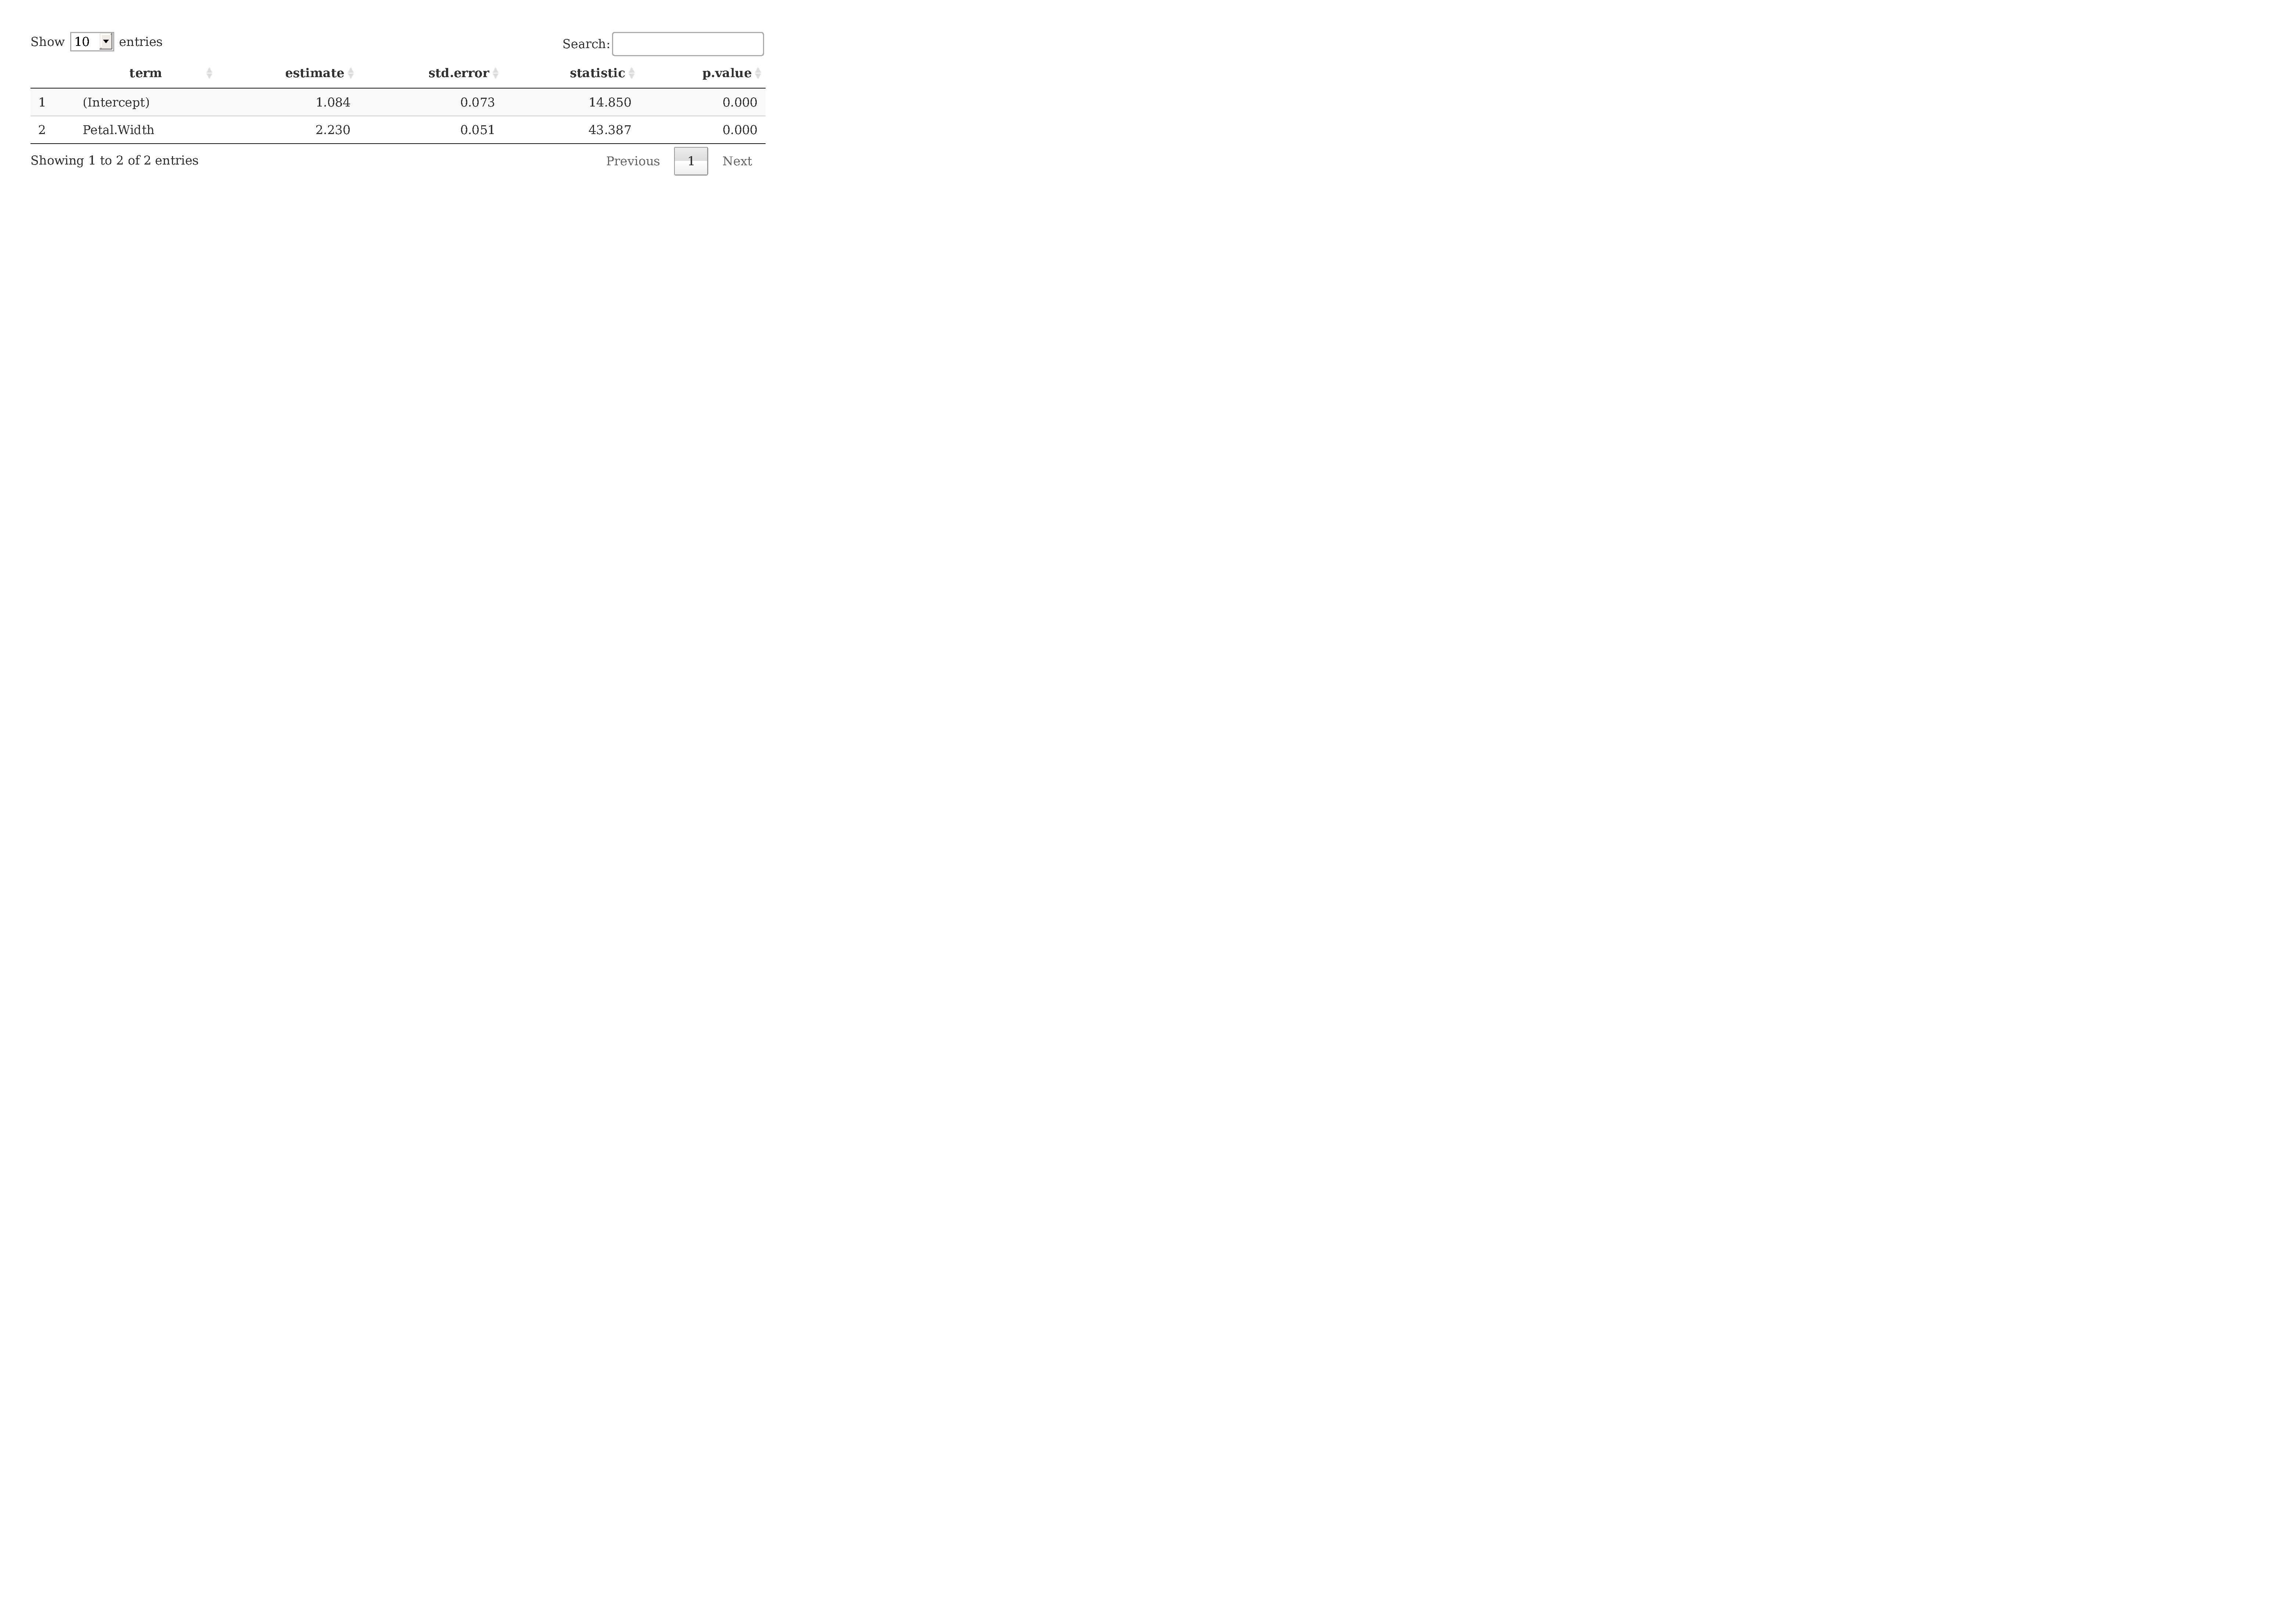
\includegraphics{functions_R_files/figure-beamer/unnamed-chunk-3-1.pdf}
\end{frame}

\begin{frame}[fragile]
\begin{block}{When should you write a function?}
\protect\hypertarget{when-should-you-write-a-function}{}
You should consider writing a function whenever you've copied and pasted
a block of code more than twice

\begin{Shaded}
\begin{Highlighting}[]
\NormalTok{a }\OtherTok{\textless{}{-}} \FunctionTok{rnorm}\NormalTok{(}\DecValTok{10}\NormalTok{)}
\NormalTok{b }\OtherTok{\textless{}{-}} \FunctionTok{rnorm}\NormalTok{(}\DecValTok{10}\NormalTok{)}
\NormalTok{c }\OtherTok{\textless{}{-}} \FunctionTok{rnorm}\NormalTok{(}\DecValTok{10}\NormalTok{)}
\NormalTok{d }\OtherTok{\textless{}{-}} \FunctionTok{rnorm}\NormalTok{(}\DecValTok{10}\NormalTok{)}
\end{Highlighting}
\end{Shaded}
\end{block}
\end{frame}

\begin{frame}[fragile]
\begin{block}{Without functions}
\protect\hypertarget{without-functions}{}
\begin{itemize}
\tightlist
\item
  introduce NA's
\end{itemize}

\begin{Shaded}
\begin{Highlighting}[]
\NormalTok{a }\SpecialCharTok{{-}} \FunctionTok{min}\NormalTok{(a)}\SpecialCharTok{/}\NormalTok{(}\FunctionTok{max}\NormalTok{(a) }\SpecialCharTok{{-}} \FunctionTok{min}\NormalTok{(a))}
\end{Highlighting}
\end{Shaded}

\begin{verbatim}
 [1]  1.0850380 -0.9344196  1.1778495 -0.4991346  1.1269565  0.2063312
 [7]  1.3443221 -0.2263243  0.4247312 -0.3406209
\end{verbatim}

\begin{Shaded}
\begin{Highlighting}[]
\NormalTok{b }\SpecialCharTok{{-}} \FunctionTok{min}\NormalTok{(b)}\SpecialCharTok{/}\NormalTok{(}\FunctionTok{max}\NormalTok{(b) }\SpecialCharTok{{-}} \FunctionTok{min}\NormalTok{(b))}
\end{Highlighting}
\end{Shaded}

\begin{verbatim}
 [1]  0.83157792  2.90539167  0.05816795  0.99407597 -1.17015769  0.36706530
 [7]  2.05683491  0.93493848  0.02653558  1.09506788
\end{verbatim}

\begin{Shaded}
\begin{Highlighting}[]
\NormalTok{c }\SpecialCharTok{{-}} \FunctionTok{min}\NormalTok{(c)}\SpecialCharTok{/}\NormalTok{(}\FunctionTok{max}\NormalTok{(c) }\SpecialCharTok{{-}} \FunctionTok{min}\NormalTok{(c))}
\end{Highlighting}
\end{Shaded}

\begin{verbatim}
 [1]  1.1305105 -1.0046556  0.4513041  0.5448090  0.6483427  0.3537967
 [7]  1.2563334  1.8417489  0.4681572 -0.7981355
\end{verbatim}

\begin{Shaded}
\begin{Highlighting}[]
\NormalTok{d }\SpecialCharTok{{-}} \FunctionTok{min}\NormalTok{(d)}\SpecialCharTok{/}\NormalTok{(}\FunctionTok{max}\NormalTok{(d) }\SpecialCharTok{{-}} \FunctionTok{min}\NormalTok{(d))}
\end{Highlighting}
\end{Shaded}

\begin{verbatim}
 [1]  0.7325955  2.4799616  1.1619310 -1.3444943  0.1501781  0.1353270
 [7] -0.4799869  0.5455207  0.1549206  1.4196076
\end{verbatim}
\end{block}
\end{frame}

\begin{frame}[fragile]
\begin{block}{Function to work on this}
\protect\hypertarget{function-to-work-on-this}{}
\begin{itemize}
\tightlist
\item
  can introduce many features applied to all
\end{itemize}

\begin{Shaded}
\begin{Highlighting}[]
\NormalTok{zero\_one }\OtherTok{\textless{}{-}} \ControlFlowTok{function}\NormalTok{(x, }\AttributeTok{na\_rm =}\NormalTok{ T, }\AttributeTok{round\_digits =} \DecValTok{3}\NormalTok{)\{}
\NormalTok{  min\_x }\OtherTok{=} \FunctionTok{min}\NormalTok{(x, }\AttributeTok{na.rm =}\NormalTok{ na\_rm)}
\NormalTok{  max\_x }\OtherTok{=} \FunctionTok{max}\NormalTok{(x, }\AttributeTok{na.rm =}\NormalTok{ na\_rm)}
\NormalTok{  diff\_x }\OtherTok{=}\NormalTok{ max\_x }\SpecialCharTok{{-}}\NormalTok{ min\_x}
\NormalTok{  ans }\OtherTok{=}\NormalTok{ (x }\SpecialCharTok{{-}}\NormalTok{ min\_x)}\SpecialCharTok{/}\NormalTok{diff\_x}
  \FunctionTok{round}\NormalTok{(ans, }\AttributeTok{digits =}\NormalTok{ round\_digits)}
\NormalTok{\}}
\end{Highlighting}
\end{Shaded}
\end{block}
\end{frame}

\begin{frame}[fragile]
\begin{block}{With Functions}
\protect\hypertarget{with-functions}{}
\begin{Shaded}
\begin{Highlighting}[]
\FunctionTok{zero\_one}\NormalTok{(a)}
\end{Highlighting}
\end{Shaded}

\begin{verbatim}
 [1] 0.886 0.000 0.927 0.191 0.905 0.501 1.000 0.311 0.596 0.261
\end{verbatim}

\begin{Shaded}
\begin{Highlighting}[]
\FunctionTok{zero\_one}\NormalTok{(b)}
\end{Highlighting}
\end{Shaded}

\begin{verbatim}
 [1] 0.491 1.000 0.301 0.531 0.000 0.377 0.792 0.517 0.294 0.556
\end{verbatim}

\begin{Shaded}
\begin{Highlighting}[]
\FunctionTok{zero\_one}\NormalTok{(c)}
\end{Highlighting}
\end{Shaded}

\begin{verbatim}
 [1] 0.750 0.000 0.512 0.544 0.581 0.477 0.794 1.000 0.517 0.073
\end{verbatim}

\begin{Shaded}
\begin{Highlighting}[]
\FunctionTok{zero\_one}\NormalTok{(d)}
\end{Highlighting}
\end{Shaded}

\begin{verbatim}
 [1] 0.543 1.000 0.655 0.000 0.391 0.387 0.226 0.494 0.392 0.723
\end{verbatim}
\end{block}

\begin{block}{Return value}
\protect\hypertarget{return-value}{}
\begin{Shaded}
\begin{Highlighting}[]
\NormalTok{plus\_one }\OtherTok{\textless{}{-}} \ControlFlowTok{function}\NormalTok{(x)\{}
\NormalTok{  x }\OtherTok{=}\NormalTok{ x}\SpecialCharTok{+}\DecValTok{1}
\NormalTok{\}}
\FunctionTok{plus\_one}\NormalTok{(}\DecValTok{5}\NormalTok{)}
\end{Highlighting}
\end{Shaded}
\end{block}
\end{frame}

\begin{frame}[fragile]
\begin{Shaded}
\begin{Highlighting}[]
\NormalTok{plus\_one\_return }\OtherTok{\textless{}{-}} \ControlFlowTok{function}\NormalTok{(x)\{}
\NormalTok{  x }\OtherTok{=}\NormalTok{ x}\SpecialCharTok{+}\DecValTok{1}
\NormalTok{  x}
\NormalTok{\}}
\FunctionTok{plus\_one\_return}\NormalTok{(}\DecValTok{5}\NormalTok{)}
\end{Highlighting}
\end{Shaded}

\begin{verbatim}
[1] 6
\end{verbatim}

\begin{Shaded}
\begin{Highlighting}[]
\NormalTok{plus\_one\_return }\OtherTok{\textless{}{-}} \ControlFlowTok{function}\NormalTok{(x)\{}
\NormalTok{  x }\OtherTok{=}\NormalTok{ x}\SpecialCharTok{+}\DecValTok{1}
  \FunctionTok{return}\NormalTok{(x)}
\NormalTok{\}}
\FunctionTok{plus\_one\_return}\NormalTok{(}\DecValTok{5}\NormalTok{)}
\end{Highlighting}
\end{Shaded}

\begin{verbatim}
[1] 6
\end{verbatim}
\end{frame}

\begin{frame}[fragile]
\begin{block}{Inputs to functions}
\protect\hypertarget{inputs-to-functions}{}
\begin{itemize}
\tightlist
\item
  Most functions require some sort of input to determine what to
  compute. The inputs to functions are called arguments. You specify
  them inside the parentheses after the word ``function.''
\item
  In the above a, b, c, d are the arguments
\end{itemize}
\end{block}

\begin{block}{Multiple inputs to functions}
\protect\hypertarget{multiple-inputs-to-functions}{}
\begin{itemize}
\tightlist
\item
  If has more than one argument, list them in the function signature,
  separated by commas.
\end{itemize}

\begin{Shaded}
\begin{Highlighting}[]
\FunctionTok{cor}\NormalTok{(}\AttributeTok{x =}\NormalTok{ iris}\SpecialCharTok{$}\NormalTok{Sepal.Length,}\AttributeTok{y=}\NormalTok{ iris}\SpecialCharTok{$}\NormalTok{Petal.Length)}
\end{Highlighting}
\end{Shaded}

\begin{verbatim}
[1] 0.8717538
\end{verbatim}
\end{block}
\end{frame}

\begin{frame}[fragile]
\begin{Shaded}
\begin{Highlighting}[]
\NormalTok{fx }\OtherTok{\textless{}{-}} \ControlFlowTok{function}\NormalTok{(x)\{}
\NormalTok{  x }\OtherTok{=}\NormalTok{ x}\SpecialCharTok{+}\DecValTok{1}
  \FunctionTok{cat}\NormalTok{(}\StringTok{"x = "}\NormalTok{, x)}
\NormalTok{  x}
\NormalTok{\}}
\end{Highlighting}
\end{Shaded}

\begin{block}{Numeric defaults}
\protect\hypertarget{numeric-defaults}{}
\begin{itemize}
\tightlist
\item
  add cutpoint = 6
\end{itemize}

\begin{Shaded}
\begin{Highlighting}[]
\NormalTok{number\_greater }\OtherTok{\textless{}{-}} \ControlFlowTok{function}\NormalTok{(age, cutpoint)\{}
\NormalTok{  age\_cut }\OtherTok{\textless{}{-}}\NormalTok{ age}\SpecialCharTok{\textgreater{}=}\NormalTok{cutpoint}
\NormalTok{  no\_greater }\OtherTok{\textless{}{-}} \FunctionTok{sum}\NormalTok{(age\_cut)}
  \FunctionTok{return}\NormalTok{(no\_greater)}
  
\NormalTok{\}}

\NormalTok{age }\OtherTok{\textless{}{-}} \FunctionTok{rnorm}\NormalTok{(}\DecValTok{100}\NormalTok{, }\AttributeTok{mean =} \DecValTok{6}\NormalTok{, }\AttributeTok{sd =} \DecValTok{3}\NormalTok{)}

\FunctionTok{number\_greater}\NormalTok{(}\AttributeTok{age =}\NormalTok{ age, }\AttributeTok{cutpoint =} \DecValTok{6}\NormalTok{)}
\end{Highlighting}
\end{Shaded}

\begin{verbatim}
[1] 43
\end{verbatim}

\begin{Shaded}
\begin{Highlighting}[]
\NormalTok{number\_greater }\OtherTok{\textless{}{-}} \ControlFlowTok{function}\NormalTok{(age, }\AttributeTok{cutpoint =} \DecValTok{6}\NormalTok{)\{}
\NormalTok{  age\_cut }\OtherTok{\textless{}{-}}\NormalTok{ age}\SpecialCharTok{\textgreater{}=}\NormalTok{cutpoint}
\NormalTok{  no\_greater }\OtherTok{\textless{}{-}} \FunctionTok{sum}\NormalTok{(age\_cut)}
  \FunctionTok{return}\NormalTok{(no\_greater)}
  
\NormalTok{\}}

\FunctionTok{number\_greater}\NormalTok{(}\AttributeTok{age =}\NormalTok{ age)}
\end{Highlighting}
\end{Shaded}

\begin{verbatim}
[1] 43
\end{verbatim}

\begin{Shaded}
\begin{Highlighting}[]
\FunctionTok{number\_greater}\NormalTok{(}\AttributeTok{age =}\NormalTok{ age, }\AttributeTok{cutpoint =} \DecValTok{7}\NormalTok{)}
\end{Highlighting}
\end{Shaded}

\begin{verbatim}
[1] 29
\end{verbatim}
\end{block}
\end{frame}

\begin{frame}[fragile]
\begin{Shaded}
\begin{Highlighting}[]
\NormalTok{x }\OtherTok{=} \DecValTok{3}
\NormalTok{z }\OtherTok{=} \FunctionTok{fx}\NormalTok{(x)}
\end{Highlighting}
\end{Shaded}

\begin{verbatim}
x =  4
\end{verbatim}

\begin{Shaded}
\begin{Highlighting}[]
\FunctionTok{cat}\NormalTok{(}\StringTok{\textquotesingle{}z =\textquotesingle{}}\NormalTok{, z)}
\end{Highlighting}
\end{Shaded}

\begin{verbatim}
z = 4
\end{verbatim}

\begin{Shaded}
\begin{Highlighting}[]
\FunctionTok{cat}\NormalTok{(}\StringTok{\textquotesingle{}x =\textquotesingle{}}\NormalTok{, x)}
\end{Highlighting}
\end{Shaded}

\begin{verbatim}
x = 3
\end{verbatim}
\end{frame}

\begin{frame}
\end{frame}



\end{document}
